\documentclass[11pt]{article}

\usepackage[margin=1in]{geometry}
\usepackage{amsmath,amssymb,amsfonts,mathtools}
\usepackage{booktabs}
\usepackage{array}
\usepackage{enumitem}
\usepackage{hyperref}
\usepackage{xcolor}
\usepackage{microtype}
\usepackage{tikz}
\usetikzlibrary{arrows.meta,positioning,calc,matrix,decorations.pathreplacing}

\hypersetup{
  colorlinks=true,
  linkcolor=blue!55!black,
  urlcolor=blue!55!black,
  citecolor=blue!55!black
}

\newcommand{\R}{\mathbb R}
\newcommand{\V}{\mathcal V}
\newcommand{\E}{\mathcal E}
\newcommand{\darts}{\overrightarrow{\mathcal E}}
\newcommand{\N}{\mathcal N}
\newcommand{\F}{\mathcal F}
\newcommand{\D}{\mathrm D}
\newcommand{\T}{\mathcal T}
\newcommand{\Hess}{\mathcal H}
\newcommand{\norm}[1]{\left\lVert #1 \right\rVert}
\newcommand{\argmin}{\operatorname*{arg\,min}}
\newcommand{\dist}{\operatorname{dist}}
\newcommand{\rank}{\operatorname{rank}}
\providecommand{\reportbuilddatetime}{unknown}
\InputIfFileExists{transported_graph_hessian_trend_filtering_build_info.tex}{}{}

\title{Transported Graph Hessian Trend Filtering}
\author{\texttt{gflow} graph trend filtering project notes}
\date{Build \reportbuilddatetime}

\begin{document}
\maketitle

\begin{abstract}
This note develops a graph trend-filtering formulation based on directional
fibers and a graph connection.  The starting point is the oriented incidence
operator, viewed not only as an edge-difference matrix but as a collection of
directional derivatives attached to each vertex.  To define a graph Hessian, one
must compare directional derivatives at neighboring vertices.  That comparison
is not well-defined from edge lengths alone: a direction at one vertex must be
matched or transported to a direction at the neighboring vertex.  We therefore
separate the construction into two pieces: a first-difference fiber
\(\F_u(f)\), and a transport rule \(T_{u\to u'}\) between neighboring fibers.
The resulting transported second difference is a graph analogue of a Hessian,
and its \(\ell_1\) norm gives a locally adaptive trend-filtering penalty.
\end{abstract}

\section{Motivation}

One-dimensional trend filtering is powerful because its penalty has a clear
calculus interpretation.  If \(f\) is sampled on a path graph, then penalizing
second differences encourages piecewise-linear behavior, and penalizing third
differences encourages piecewise-quadratic behavior.  Algebraically, the
unpenalized space is the null space of a finite-difference operator.  For
example, on a connected path,
\[
  \D^2 f = 0
  \quad\Longleftrightarrow\quad
  f \text{ is affine along the path},
\]
and
\[
  \D^3 f = 0
  \quad\Longleftrightarrow\quad
  f \text{ is quadratic along the path}.
\]

For a graph that samples a two- or three-dimensional domain, a purely
pathwise construction is useful but incomplete.  It asks whether \(f\) looks
polynomial along selected geodesics.  A more multivariate construction should
ask whether the graph has a meaningful analogue of a gradient, Hessian, and
higher derivative tensor.

The first graph derivative is already available: the oriented incidence
operator.  The new question is how to differentiate it again.  That is the
central issue of this document.

\begin{center}
\begin{minipage}{0.86\linewidth}
\itshape
Edge lengths define how far apart adjacent vertices are.  A graph Hessian also
needs to know which edge directions at neighboring vertices should be compared.
That extra datum is a discrete connection or parallel-transport rule.
\end{minipage}
\end{center}

\section{Metric Graphs, Darts, and Directional Fibers}

Let
\[
  G=(\V,\E,\ell)
\]
be an undirected graph with positive edge lengths \(\ell_{uv}>0\).  Instead of
choosing one global orientation per edge, it is convenient to use both directed
versions of every edge:
\[
  \darts
  =
  \{u\to v:\{u,v\}\in\E\}.
\]
We call these directed edges \emph{darts}.  For a function
\[
  f:\V\to\R,
\]
define the length-normalized directional difference along the dart \(u\to v\):
\[
  \delta_{u\to v}f
  =
  \frac{f(v)-f(u)}{\ell_{uv}}.
\]

The first-difference fiber at \(u\) is the vector of outgoing directional
differences:
\[
  \F_u(f)
  =
  \bigl(\delta_{u\to v}f\bigr)_{v\in\N(u)}
  \in \R^{\N(u)}.
\]
This is a graph analogue of the directional derivative of \(f\) in every
available outgoing edge direction.

\begin{figure}[ht]
\centering
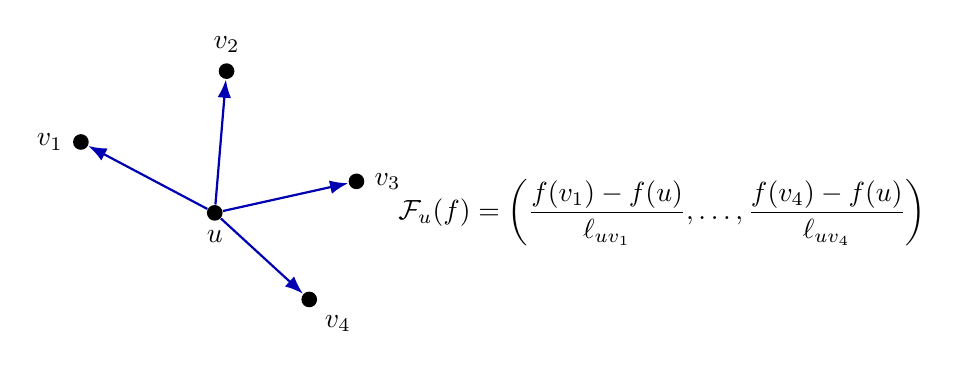
\begin{tikzpicture}[>=Latex,scale=1.0]
  \node[circle,fill=black,inner sep=2pt,label=below:{\(u\)}] (u) at (0,0) {};
  \node[circle,fill=black,inner sep=2pt,label=left:{\(v_1\)}] (v1) at (-1.7,0.9) {};
  \node[circle,fill=black,inner sep=2pt,label=above:{\(v_2\)}] (v2) at (0.15,1.8) {};
  \node[circle,fill=black,inner sep=2pt,label=right:{\(v_3\)}] (v3) at (1.8,0.4) {};
  \node[circle,fill=black,inner sep=2pt,label=below right:{\(v_4\)}] (v4) at (1.2,-1.1) {};
  \draw[thick,->,blue!70!black] (u) -- (v1);
  \draw[thick,->,blue!70!black] (u) -- (v2);
  \draw[thick,->,blue!70!black] (u) -- (v3);
  \draw[thick,->,blue!70!black] (u) -- (v4);
  \node[align=left,right=2.1cm of u] {
    \(\displaystyle \F_u(f)=
    \left(
    \frac{f(v_1)-f(u)}{\ell_{uv_1}},
    \ldots,
    \frac{f(v_4)-f(u)}{\ell_{uv_4}}
    \right)\)
  };
\end{tikzpicture}
\caption{The first-difference fiber at a vertex is the collection of
length-normalized outgoing differences.  It is the discrete object that plays
the role of a local directional gradient.}
\end{figure}

\section{Why Raw All-Pairs Fiber Differences Are Too Strong}

A tempting second-difference construction is to compare every outgoing
directional derivative at \(u'\) with every outgoing directional derivative at
\(u\) across a base dart \(u\to u'\).  This gives entries of the form
\[
  \delta_{u'\to v'}f-\delta_{u\to v}f,
  \qquad
  v\in\N(u),\quad v'\in\N(u').
\]
This is mathematically definable, but it is not the graph Hessian we want.  It
compares unrelated directional derivatives.

The problem already appears on a square grid.  Orient local directions by the
coordinate axes and take
\[
  f(i,j)=i.
\]
Then
\[
  \Delta_x f = 1,
  \qquad
  \Delta_y f = 0.
\]
An all-pairs comparison includes terms such as
\[
  \Delta_y f(i+1,j)-\Delta_x f(i,j)=0-1=-1.
\]
Thus a raw all-pairs second-difference penalty would not annihilate an affine
function on a grid.  A graph Hessian should annihilate affine functions.

\begin{figure}[ht]
\centering
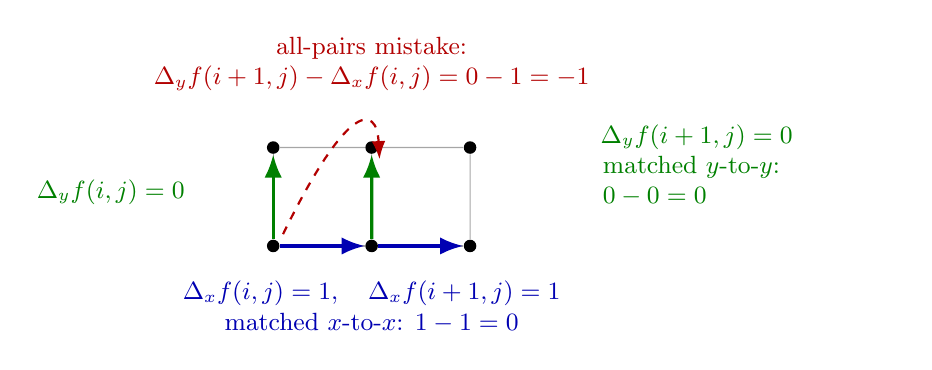
\begin{tikzpicture}[>=Latex,scale=1.25,every node/.style={font=\small}]
  \foreach \x in {0,1,2} {
    \foreach \y in {0,1} {
      \node[circle,fill=black,inner sep=1.6pt] (p\x\y) at (\x,\y) {};
    }
  }
  \draw[gray!70] (p00)--(p10)--(p20);
  \draw[gray!70] (p01)--(p11)--(p21);
  \draw[gray!70] (p00)--(p01);
  \draw[gray!70] (p10)--(p11);
  \draw[gray!70] (p20)--(p21);

  \draw[very thick,->,blue!70!black] (p00) -- (p10);
  \draw[very thick,->,blue!70!black] (p10) -- (p20);
  \draw[very thick,->,green!50!black] (p10) -- (p11);
  \draw[very thick,->,green!50!black] (p00) -- (p01);

  \draw[red!70!black,thick,dashed,->]
    ($(p00)+(0.10,0.12)$) .. controls (0.75,1.45) and (1.05,1.45) .. ($(p10)+(0.08,0.88)$);

  \node[blue!70!black,align=center] at (1.0,-0.62)
    {\(\Delta_x f(i,j)=1,\quad \Delta_x f(i+1,j)=1\)\\
     matched \(x\)-to-\(x\): \(1-1=0\)};
  \node[green!50!black,align=right] at (-1.65,0.55)
    {\(\Delta_y f(i,j)=0\)};
  \node[green!50!black,align=left,anchor=west,text width=3.7cm] at (3.25,0.82)
    {\(\Delta_y f(i+1,j)=0\)\\
     matched \(y\)-to-\(y\):\\
     \(0-0=0\)};
  \node[red!70!black,align=center] at (1.0,1.85)
    {all-pairs mistake:\\ \(\Delta_y f(i+1,j)-\Delta_x f(i,j)=0-1=-1\)};
\end{tikzpicture}
\caption{On a grid, all-pairs fiber comparison mixes unrelated directions.
For \(f(i,j)=i\), comparing a \(y\)-direction derivative with an \(x\)-direction
derivative produces a nonzero second difference even though \(f\) is affine.}
\end{figure}

This example shows why a second derivative needs a direction-matching rule.
In smooth geometry, directional derivatives at neighboring points are compared
after parallel transport.  The graph version needs the same idea.

\section{The Abstract Transported Graph Hessian}

Let \(a=u\to u'\) be a base dart.  A direction-transport rule assigns a matrix
\[
  T_{u\to u'}:\R^{\N(u')}\to\R^{\N(u)}.
\]
The entry \(T_{u\to u'}(v,v')\) describes how much the outgoing direction
\(u'\to v'\) contributes to the transported version of the direction
\(u\to v\).

The transported second difference is
\[
  \bigl(\D_T^2 f\bigr)_{u\to u'}(v)
  =
  \sum_{v'\in\N(u')}
  T_{u\to u'}(v,v')\,\delta_{u'\to v'}f
  -
  \delta_{u\to v}f.
\]
Equivalently,
\[
  \D_T^2 f(u\to u')
  =
  T_{u\to u'}\F_{u'}(f)-\F_u(f).
\]

This is the graph-Hessian object.  It compares the directional fiber at
\(u'\) with the directional fiber at \(u\), but only after transporting the
\(u'\)-fiber into the \(u\)-fiber.  The construction is linear in \(f\) as long
as the transport matrices are built from the graph geometry and held fixed
during fitting.

\begin{figure}[ht]
\centering
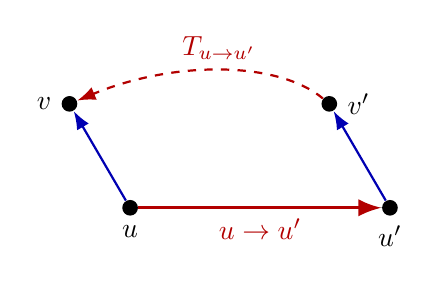
\begin{tikzpicture}[>=Latex,scale=1.1]
  \node[circle,fill=black,inner sep=2pt,label=below:{\(u\)}] (u) at (0,0) {};
  \node[circle,fill=black,inner sep=2pt,label=below:{\(u'\)}] (up) at (3,0) {};
  \node[circle,fill=black,inner sep=2pt,label=left:{\(v\)}] (v) at (-0.7,1.2) {};
  \node[circle,fill=black,inner sep=2pt,label=right:{\(v'\)}] (vp) at (2.3,1.2) {};

  \draw[gray!65] (u)--(up);
  \draw[thick,->,blue!70!black] (u)--(v);
  \draw[thick,->,blue!70!black] (up)--(vp);
  \draw[very thick,->,red!70!black] (u) -- node[below] {\(u\to u'\)} (up);
  \draw[red!70!black,dashed,thick,->] (vp) .. controls (1.7,1.7) and (0.5,1.7) .. node[above] {\(T_{u\to u'}\)} (v);
\end{tikzpicture}
\caption{The transported Hessian compares outgoing directional derivatives
after a direction at \(u'\) has been matched or transported to a direction at
\(u\).  The transport matrix is the extra structure missing from an edge-length
only graph.}
\end{figure}

\section{Direction-Matching and Parallel-Transport Rules}

The abstract operator is only useful after specifying \(T_{u\to u'}\).  This
section lists transport rules that are compatible with the graph-trend-filtering
project.  They range from exact grid references to geometry-estimated soft
matching.

\subsection{Exact Coordinate Matching}

On a coordinate grid, each dart has a coordinate direction label:
\[
  +x,\ -x,\ +y,\ -y,\ldots.
\]
For a base dart \(u\to u'\), define
\[
  T_{u\to u'}(v,v')=
  \begin{cases}
    1, & \text{if } u\to v \text{ and } u'\to v'
         \text{ have the same coordinate direction},\\
    0, & \text{otherwise}.
  \end{cases}
\]

This rule recovers ordinary finite-difference Hessian entries on a lattice.
It is the first implementation reference because the expected null spaces are
known:
\[
  \D^1 f=0 \Longleftrightarrow f \text{ is constant},
  \qquad
  \D_T^2 f=0 \Longleftrightarrow f \text{ is affine}
\]
on a connected rectangular grid, away from boundary conventions.

\subsection{Edge-Angle Riemannian Graph Matching}

Suppose the graph has been enriched with angles between incident edges.  For
neighbors \(v,w\in\N(u)\), let
\[
  \cos\theta_u(v,w)
\]
be the cosine of the angle between the darts \(u\to v\) and \(u\to w\).
Across a base dart \(u\to u'\), the direction \(u'\to v'\) should match
\(u\to v\) when both have similar orientation relative to the base edge.  Since
the base direction reverses when viewed from \(u'\), one natural mismatch score
is
\[
  S_{u\to u'}(v,v')
  =
  \left|
  \cos\theta_u(v,u')
  +
  \cos\theta_{u'}(v',u)
  \right|.
\]
Small \(S\) means that the two directions make compatible angles with the
base edge.

A hard matching chooses the best \(v'\) for each \(v\), but only if the match
is good enough.  Thus a hard rule should include an acceptance threshold:
\[
  v^\star(v)
  =
  \argmin_{v'\in\N(u')} S_{u\to u'}(v,v'),
  \qquad
  T_{u\to u'}(v,v^\star)=1
  \quad\text{only if}\quad
  S_{u\to u'}(v,v^\star)\le s_{\max}.
\]
If the best score is larger than \(s_{\max}\), that direction is left
unmatched or handled by a boundary/sparse-neighborhood rule.  The threshold
\(s_{\max}\) is therefore the main modeling choice in hard matching.

A soft matching uses
\[
  T_{u\to u'}(v,v')
  =
  \frac{\exp\{-S_{u\to u'}(v,v')^2/\tau^2\}}
       {\sum_{w\in\N(u')}\exp\{-S_{u\to u'}(v,w)^2/\tau^2\}}.
\]
The bandwidth \(\tau\) controls how sharply directions are matched.  In
practice \(\tau\) should be chosen from the empirical distribution of available
nonzero mismatch scores.  A robust default is
\[
  \tau
  =
  c_\tau\,
  \operatorname{median}
  \{S_{u\to u'}(v,v'):\text{candidate pairs in local disks}\},
\]
with \(c_\tau\in[0.5,1]\).  A more local version uses the median score inside
the current disk or for the current base dart.  The effective entropy of each
row of \(T\) should be reported: if all mass falls on one direction, the rule
is nearly hard matching; if the mass is almost uniform, \(\tau\) is too large.

This rule is close to the earlier idea of enriching a weighted graph into a
Riemannian graph: edge lengths give metric scale, and incident-edge angles give
local tangent geometry.

\subsection{Local Embedding Soft Transport}

When angles are not given, we can estimate them in local coordinates.  For a
base dart \(u\to u'\), choose a graph disk containing \(u\), \(u'\), and their
neighbors.  Embed this disk in \(\R^m\) using a local coordinate method such as
metric MDS or weighted-GRIP followed by edge-KK refinement.  Let \(z_w\) denote
the local coordinate of vertex \(w\).

Define unit edge directions
\[
  \xi_u(v)=
  \frac{z_v-z_u}{\norm{z_v-z_u}},
  \qquad
  \xi_{u'}(v')=
  \frac{z_{v'}-z_{u'}}{\norm{z_{v'}-z_{u'}}}.
\]
If both fibers are represented in the same local chart, then
\[
  T_{u\to u'}(v,v')
  =
  \frac{
  \exp\{-\norm{\xi_u(v)-\xi_{u'}(v')}^2/(2\sigma_\theta^2)\}
  }
  {
  \sum_{w\in\N(u')}
  \exp\{-\norm{\xi_u(v)-\xi_{u'}(w)}^2/(2\sigma_\theta^2)\}
  }.
\]

If separate charts are used at \(u\) and \(u'\), first align the overlapping
vertices by an orthogonal Procrustes map.  This makes the rule a discrete
parallel transport induced by local coordinate frames.

The bandwidth \(\sigma_\theta\) is the angular analogue of \(\tau\).  Since
\(\xi_u(v)\) and \(\xi_{u'}(v')\) are unit vectors,
\[
  \norm{\xi_u(v)-\xi_{u'}(v')}^2
  =
  2\{1-\cos\angle(\xi_u(v),\xi_{u'}(v'))\}.
\]
Therefore \(\sigma_\theta\) can be specified as an angular bandwidth.  If a
typical acceptable angular mismatch is \(\alpha_0\), set
\[
  \sigma_\theta^2 = 2(1-\cos\alpha_0).
\]
For example, \(\alpha_0=20^\circ\) gives a fairly sharp match, while
\(\alpha_0=35^\circ\) is more forgiving.  A data-adaptive alternative is to set
\(\sigma_\theta\) to the median nearest-neighbor directional mismatch among
candidate direction pairs in the local disk.

This is the most practical rule for data-derived kNN graphs.  It accepts that
high-degree neighborhoods contain many sampled directions and uses soft
matching rather than forcing one-to-one correspondences.

\subsection{Adaptive Local Transport Thresholding}

The soft transport rule assigns weights to candidate directions, but the
operator still needs to decide whether a transported comparison is trustworthy
enough to become a Hessian row.  A fixed global threshold is often too crude.
The same numerical margin can mean different things at a path endpoint, a grid
interior vertex, and a high-degree \(k\)-NN neighborhood.  The practical rule
should therefore judge a candidate match relative to the local score
distribution available at the current transported fiber.

For a base dart \(u\to u'\), a source direction \(u\to v\), and target
candidates \(u'\to v'_j\), write
\[
  s_j = S_{u\to u'}(v,v'_j),
  \qquad j=1,\ldots,J,
\]
and let
\[
  s_{(1)}\le s_{(2)}\le\cdots\le s_{(J)}
\]
be the ordered scores.  The best candidate is useful only when it is locally
good and locally separated from the alternatives.  The best-versus-second
margin is
\[
  m = s_{(2)}-s_{(1)}.
\]

\paragraph{Local quantile rule.}
Let \(\widehat F_s\) be the empirical distribution function of the local
candidate scores and let \(\widehat F_{\Delta s}\) be the empirical
distribution function of the adjacent score gaps
\[
  \Delta s_j=s_{(j+1)}-s_{(j)},\qquad j=1,\ldots,J-1.
\]
Define
\[
  q_s = \widehat F_s(s_{(1)}),
  \qquad
  q_m = \widehat F_{\Delta s}(m).
\]
A local quantile gate accepts the row only if
\[
  q_s\le q_{\max},
  \qquad
  q_m\ge q_{\min}.
\]
The first inequality says that the best score is in the lower tail of the
local score distribution.  The second says that the best score is separated
from the runner-up by a locally meaningful gap.

\paragraph{Local robust-\(z\) rule.}
An alternative is to measure the same two ideas using robust local scales.
Let
\[
  \operatorname{scale}(x)
  =
  1.4826\,\operatorname{MAD}(x)
\]
with fallback to interquartile range or standard deviation when the median
absolute deviation is zero.  Define
\[
  z_s
  =
  \frac{\operatorname{median}(s)-s_{(1)}}
       {\operatorname{scale}(s)},
  \qquad
  z_m
  =
  \frac{m-\operatorname{median}(\Delta s)}
       {\operatorname{scale}(\Delta s)}.
\]
A robust-\(z\) gate accepts the row only if
\[
  z_s\ge z_{s,\min},
  \qquad
  z_m\ge z_{m,\min}.
\]
Large \(z_s\) means the best candidate is unusually good relative to the local
candidate cloud.  Large \(z_m\) means the best candidate is unusually well
separated from the next best candidate.

\paragraph{Entropy-fraction rule.}
The softmax weights
\[
  w_j
  =
  \frac{\exp\{-s_j^2/\tau^2\}}
       {\sum_{k=1}^J\exp\{-s_k^2/\tau^2\}}
\]
also provide a useful ambiguity diagnostic.  Define the softmax entropy
\[
  H=-\sum_{j=1}^J w_j\log w_j,
\]
the effective number of matched directions
\[
  n_{\mathrm{eff}}=\exp(H),
\]
and the local effective-match fraction
\[
  \rho_H=\frac{n_{\mathrm{eff}}}{J}.
\]
The fraction \(\rho_H\) is close to \(1/J\) when the match is concentrated on
one direction, and close to \(1\) when the match is nearly uniform.  A row can
therefore be rejected when
\[
  \rho_H>\rho_{\max}.
\]
This makes the entropy threshold comparable across vertices of different
degree.

\begin{figure}[ht]
\centering
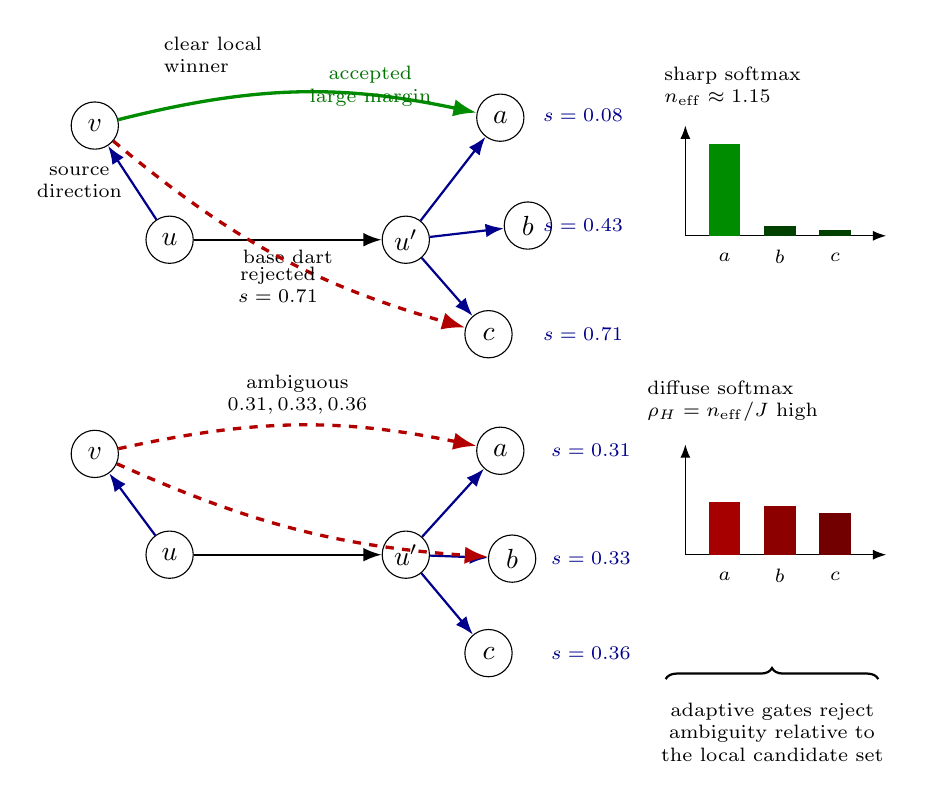
\begin{tikzpicture}[
  >=Latex,
  x=1cm,
  y=1cm,
  vertex/.style={circle,draw=black,fill=white,minimum size=6mm,inner sep=0pt},
  good/.style={draw=green!55!black,very thick},
  bad/.style={draw=red!70!black,very thick,dashed},
  candidate/.style={draw=blue!55!black,thick},
  score/.style={font=\scriptsize,align=center},
  smalltxt/.style={font=\scriptsize,align=center}
]
  \node[vertex] (u) at (0,0) {\(u\)};
  \node[vertex] (up) at (3.0,0) {\(u'\)};
  \node[vertex] (v) at (-0.95,1.45) {\(v\)};
  \node[vertex] (a) at (4.2,1.55) {\(a\)};
  \node[vertex] (b) at (4.55,0.18) {\(b\)};
  \node[vertex] (c) at (4.05,-1.20) {\(c\)};
  \draw[->,thick] (u) -- node[below,smalltxt] {base dart} (up);
  \draw[->,candidate] (u) -- node[left,smalltxt] {source\\direction} (v);
  \draw[->,candidate] (up) -- (a);
  \draw[->,candidate] (up) -- (b);
  \draw[->,candidate] (up) -- (c);
  \draw[->,good,bend left=13] (v) to (a);
  \node[score,green!45!black] at (2.55,1.95)
    {accepted\\large margin};
  \draw[->,bad,bend right=12] (v) to node[below,score]
    {rejected\\\(s=0.71\)} (c);
  \node[score,blue!55!black] at (5.25,1.58) {\(s=0.08\)};
  \node[score,blue!55!black] at (5.25,0.18) {\(s=0.43\)};
  \node[score,blue!55!black] at (5.25,-1.20) {\(s=0.71\)};
  \node[smalltxt,align=left] at (0.55,2.35)
    {clear local\\winner};

  \node[vertex] (u2) at (0,-4.0) {\(u\)};
  \node[vertex] (up2) at (3.0,-4.0) {\(u'\)};
  \node[vertex] (v2) at (-0.95,-2.72) {\(v\)};
  \node[vertex] (a2) at (4.2,-2.68) {\(a\)};
  \node[vertex] (b2) at (4.35,-4.05) {\(b\)};
  \node[vertex] (c2) at (4.05,-5.25) {\(c\)};
  \draw[->,thick] (u2) -- (up2);
  \draw[->,candidate] (u2) -- (v2);
  \draw[->,candidate] (up2) -- (a2);
  \draw[->,candidate] (up2) -- (b2);
  \draw[->,candidate] (up2) -- (c2);
  \draw[->,bad,bend left=12] (v2) to node[above,score]
    {ambiguous\\\(0.31,0.33,0.36\)} (a2);
  \draw[->,bad,bend right=10] (v2) to (b2);
  \node[score,blue!55!black] at (5.35,-2.68) {\(s=0.31\)};
  \node[score,blue!55!black] at (5.35,-4.05) {\(s=0.33\)};
  \node[score,blue!55!black] at (5.35,-5.25) {\(s=0.36\)};

  \node[smalltxt,align=left] at (7.15,1.95)
    {sharp softmax\\\(n_{\mathrm{eff}}\approx 1.15\)};
  \draw[->] (6.55,0.05) -- (9.1,0.05);
  \draw[->] (6.55,0.05) -- (6.55,1.45);
  \fill[green!55!black] (6.85,0.05) rectangle (7.25,1.22);
  \fill[green!25!black] (7.55,0.05) rectangle (7.95,0.18);
  \fill[green!25!black] (8.25,0.05) rectangle (8.65,0.12);
  \node[smalltxt] at (7.05,-0.22) {\(a\)};
  \node[smalltxt] at (7.75,-0.22) {\(b\)};
  \node[smalltxt] at (8.45,-0.22) {\(c\)};

  \node[smalltxt,align=left] at (7.15,-2.05)
    {diffuse softmax\\\(\rho_H=n_{\mathrm{eff}}/J\) high};
  \draw[->] (6.55,-4.0) -- (9.1,-4.0);
  \draw[->] (6.55,-4.0) -- (6.55,-2.6);
  \fill[red!65!black] (6.85,-4.0) rectangle (7.25,-3.33);
  \fill[red!55!black] (7.55,-4.0) rectangle (7.95,-3.38);
  \fill[red!45!black] (8.25,-4.0) rectangle (8.65,-3.47);
  \node[smalltxt] at (7.05,-4.27) {\(a\)};
  \node[smalltxt] at (7.75,-4.27) {\(b\)};
  \node[smalltxt] at (8.45,-4.27) {\(c\)};

  \draw[decorate,decoration={brace,amplitude=4pt},thick]
    (6.3,-5.58) -- node[below=5pt,smalltxt,text width=3.6cm]
    {adaptive gates reject ambiguity relative to the local candidate set}
    (9.0,-5.58);
\end{tikzpicture}
\caption{Adaptive local thresholding for transported direction matching.  The
top neighborhood has one clearly best candidate, a large margin, and a sharp
softmax distribution; it is accepted.  The bottom neighborhood has several
nearly tied candidates and diffuse softmax mass; it is rejected by local
quantile, robust-\(z\), or entropy-fraction gates.}
\label{fig:adaptive-local-transport-thresholding}
\end{figure}

These thresholds are best understood as diagnostic and experimental controls,
not as a final mathematical axiom.  They decide which transported directional
comparisons are trusted before they enter the Hessian operator.  Every accepted
or dropped row should carry the corresponding diagnostics: best score, second
score, margin, robust-\(z\) values, entropy, effective-match fraction, and drop
reason.  This keeps the operator auditable on irregular graphs.

\subsection{Status of the Adaptive-Threshold Calibration Experiment}

The first calibration sweep treated adaptive thresholding as a retention
constrained model-selection problem.  For each graph, threshold setting, and
transport backend, the experiment measured the linear-polynomial residual
\[
  R_{\mathrm{linear}}
  =
  \frac{\norm{A P_{\mathrm{linear}}}_F}
       {\norm{P_{\mathrm{linear}}}_F}
\]
subject to the practical constraint
\[
  \rho_{\mathrm{row}}
  =
  \frac{\#\{\text{accepted rows}\}}
       {\#\{\text{candidate rows}\}}
  \ge 0.50.
\]
This constraint is essential.  Very low residuals are not meaningful if they
are obtained by dropping most Hessian rows.

\begin{figure}[ht]
\centering
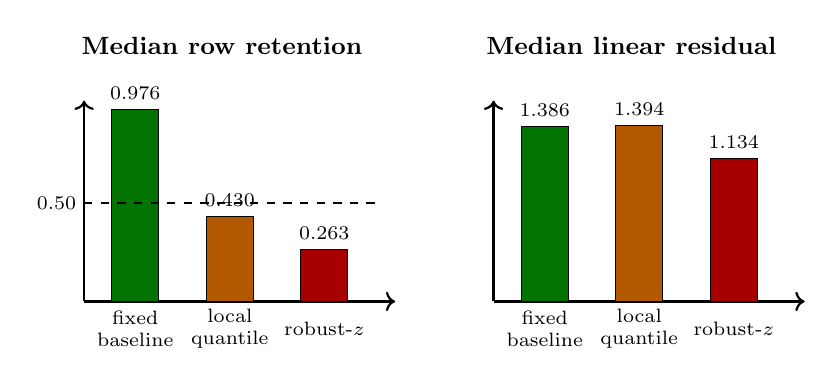
\begin{tikzpicture}[
  x=1cm,
  y=1cm,
  bar/.style={draw=black,fill=blue!35},
  txt/.style={font=\scriptsize,align=center},
  axis/.style={->,thick}
]
  \node[font=\small\bfseries] at (1.75,3.25) {Median row retention};
  \draw[axis] (0,0) -- (0,2.55);
  \draw[axis] (0,0) -- (3.95,0);
  \draw[bar,fill=green!45!black] (0.35,0) rectangle (0.95,2.44);
  \draw[bar,fill=orange!70!black] (1.55,0) rectangle (2.15,1.08);
  \draw[bar,fill=red!65!black] (2.75,0) rectangle (3.35,0.66);
  \draw[dashed,thick] (0,1.25) -- (3.75,1.25);
  \node[txt] at (-0.35,1.25) {0.50};
  \node[txt] at (0.65,-0.35) {fixed\\baseline};
  \node[txt] at (1.85,-0.35) {local\\quantile};
  \node[txt] at (3.05,-0.35) {robust-\(z\)};
  \node[txt] at (0.65,2.65) {0.976};
  \node[txt] at (1.85,1.28) {0.430};
  \node[txt] at (3.05,0.86) {0.263};

  \begin{scope}[xshift=5.2cm]
    \node[font=\small\bfseries] at (1.75,3.25) {Median linear residual};
    \draw[axis] (0,0) -- (0,2.55);
    \draw[axis] (0,0) -- (3.95,0);
    \draw[bar,fill=green!45!black] (0.35,0) rectangle (0.95,2.22);
    \draw[bar,fill=orange!70!black] (1.55,0) rectangle (2.15,2.23);
    \draw[bar,fill=red!65!black] (2.75,0) rectangle (3.35,1.81);
    \node[txt] at (0.65,-0.35) {fixed\\baseline};
    \node[txt] at (1.85,-0.35) {local\\quantile};
    \node[txt] at (3.05,-0.35) {robust-\(z\)};
    \node[txt] at (0.65,2.43) {1.386};
    \node[txt] at (1.85,2.44) {1.394};
    \node[txt] at (3.05,2.02) {1.134};
  \end{scope}
\end{tikzpicture}
\caption{Summary of the adaptive-threshold calibration sweep.  Adaptive gates
can reduce residuals, but the reduction often comes with substantial row loss.
The fixed angle/length rule remains the safest broad baseline under the
\(50\%\) row-retention constraint.}
\label{fig:adaptive-threshold-calibration-summary}
\end{figure}

The sweep tested 294 operator constructions and all runs completed.  The main
finding is not that adaptive gates are useless; rather, they are not yet a
universal default.  They won on clean path and grid references, but the fixed
angle/length gate won on jittered grids and sampled symmetric \(k\)-NN graphs.
This is exactly the pattern one would expect if local score filters are good
calibration diagnostics but can become overly aggressive on irregular real-data
graphs.

The conclusion for the next phase is therefore to stop adding more gates to
the same soft-matching rule and instead implement a qualitatively different
parallel-transport mechanism.

\subsection{Approximate Parallelogram Transport}

There is also a parallelogram idea: match \(u\to v\) with \(u'\to v'\) when the
four vertices approximately close a translated quadrilateral.  There are two
versions, and they should not be confused.

For a base dart \(u\to u'\), define
\[
  Q^{G}_{u\to u'}(v,v')
  =
  \left|d_G(v,v')-\ell_{uu'}\right|
  +
  \left|\ell_{uv}-\ell_{u'v'}\right|.
\]
Small \(Q^G\) means that \(v'\) is close to where \(v\) would be translated by
the displacement \(u\to u'\), using only graph distances.  This is an appealing
intrinsic formula, but it is also strong.  In a generic sparse graph,
\(d_G(v,v')\approx \ell_{uu'}\) may fail simply because the graph has no short
edge or short path between \(v\) and \(v'\), even when the ambient or latent
geometry says the two directions are parallel.

For data-derived kNN graphs with ambient coordinates \(x_u\), or with reliable
local isometric embedding coordinates \(z_u\), the more practical
parallelogram score is
\[
  Q^{E}_{u\to u'}(v,v')
  =
  \left|
  \norm{x_v-x_{v'}}-\norm{x_u-x_{u'}}
  \right|
  +
  \left|
  \norm{x_u-x_v}-\norm{x_{u'}-x_{v'}}
  \right|.
\]
The same formula can be used with \(z\)-coordinates instead of \(x\)-coordinates
when ambient coordinates are unavailable or when one wants an intrinsic local
embedding.  A still sharper coordinate version also checks displacement-vector
closure:
\[
  Q^{\mathrm{vec}}_{u\to u'}(v,v')
  =
  \norm{(x_{v'}-x_{u'})-(x_v-x_u)}.
\]

A soft transport can then use whichever score is appropriate:
\[
  T_{u\to u'}(v,v')
  =
  \frac{\exp\{-Q_{u\to u'}(v,v')^2/\tau_Q^2\}}
       {\sum_{w\in\N(u')}\exp\{-Q_{u\to u'}(v,w)^2/\tau_Q^2\}}.
\]
Here \(Q\) may be \(Q^G\), \(Q^E\), or \(Q^{\mathrm{vec}}\).  In practice,
\(Q^E\) or \(Q^{\mathrm{vec}}\) should be preferred for kNN graphs when
ambient coordinates are available.

\begin{figure}[ht]
\centering
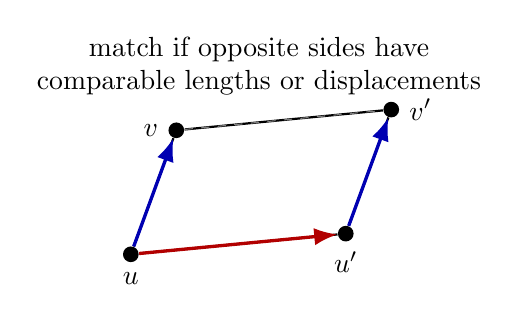
\begin{tikzpicture}[>=Latex,scale=1.05]
  \node[circle,fill=black,inner sep=2pt,label=below:{\(u\)}] (u) at (0,0) {};
  \node[circle,fill=black,inner sep=2pt,label=below:{\(u'\)}] (up) at (2.6,0.25) {};
  \node[circle,fill=black,inner sep=2pt,label=left:{\(v\)}] (v) at (0.55,1.5) {};
  \node[circle,fill=black,inner sep=2pt,label=right:{\(v'\)}] (vp) at (3.15,1.75) {};
  \draw[thick] (u)--(up)--(vp);
  \draw[thick] (u)--(v)--(vp);
  \draw[dashed,gray] (v)--(vp);
  \draw[very thick,->,blue!70!black] (u)--(v);
  \draw[very thick,->,blue!70!black] (up)--(vp);
  \draw[very thick,->,red!70!black] (u)--(up);
  \node[align=center] at (1.55,2.28) {
    match if opposite sides have\\
    comparable lengths or displacements
  };
\end{tikzpicture}
\caption{Approximate parallelogram transport matches edge directions by
asking whether the four vertices close a parallelogram.  On generic sparse
graphs, an ambient or local-embedding score is often more practical than a
pure graph-distance score.}
\end{figure}

\subsection{Regression-Based Gradient Transport}

The previous rules match individual edge directions.  A different approach is
to estimate a local gradient vector at each vertex and then compare gradients.

In local coordinates \(z_w\) around \(u\), fit
\[
  f(w)-f(u)
  \approx
  g_u^\top(z_w-z_u)
\]
by weighted least squares.  The fitted gradient is linear in \(f\):
\[
  g_u = L_u f
\]
for a matrix \(L_u\) determined by the local coordinates and weights.

The coordinates \(z_w\) may come from three sources:
\begin{enumerate}[label=(\roman*),leftmargin=*]
  \item ambient coordinates, when the graph was constructed from observed
  points \(x_w\in\R^p\);
  \item local isometric embedding coordinates from graph distances, such as
  metric MDS or weighted-GRIP followed by edge-KK refinement;
  \item coordinates supplied by an enriched Riemannian graph representation.
\end{enumerate}
For synthetic kNN benchmarks, ambient coordinates are useful for debugging.
For the intended graph-intrinsic method, the default should be local isometric
coordinates from a graph disk.

The disk radius should be chosen adaptively rather than fixed globally.  A
reasonable rule is
\[
  r_u
  =
  \min\{r:\#D_G(u,r)\ge n_{\min}
  \text{ and } \#E(D_G(u,r))\ge e_{\min}\},
\]
subject to \(r_u\le r_{\max}\).  The minimum vertex count should exceed the
number of regression coefficients.  For an \(m\)-dimensional local linear fit,
one needs at least \(m+1\) nondegenerate points, but in practice
\[
  n_{\min}\approx 3(m+1)\quad\text{to}\quad 5(m+1)
\]
is safer.  The chosen disk should also pass a conditioning check on the local
design matrix.  If the local design is ill-conditioned, the algorithm should
increase the radius, reduce the estimated local dimension, or mark the gradient
as unreliable.

Across a base dart \(u\to u'\), align the coordinate frames by a map
\(\Pi_{u'\to u}\), and define
\[
  \Hess_{u\to u'}f
  =
  \frac{\Pi_{u'\to u} g_{u'}-g_u}{\ell_{uu'}}.
\]
This is a vector-valued second difference.  It bypasses the variable degree of
graph vertices and may be the numerically cleanest way to build Hessian-like
rows on high-degree kNN graphs.

The tradeoff is conceptual: this rule is less purely incidence-based.  It is a
local regression derivative, not a direct comparison of raw edge differences.

\section{Trend-Filtering Penalties}

Once \(T\) is fixed, the transported Hessian is a linear operator in \(f\).
The order-two transported graph trend-filtering estimator is
\[
  \widehat f_\lambda
  =
  \argmin_{f\in\R^{|\V|}}
  \frac12\sum_{u\in\V}(y_u-f_u)^2
  +
  \lambda\norm{\D_T^2 f}_1.
\]
This is the \(\ell_1\)-adaptive analogue of a graph Hessian smoother.  The
\(\ell_1\) penalty encourages many transported directional-gradient changes to
be exactly zero, so the fitted signal is locally affine except across selected
graph regions where the Hessian-like quantity is allowed to jump.

If \(D^1\) denotes the length-normalized dart incidence operator, then the
first-order case is graph total variation:
\[
  \widehat f_\lambda
  =
  \argmin_f
  \frac12\norm{y-f}_2^2+\lambda\norm{D^1f}_1.
\]
The transported second-order case is the candidate graph analogue of linear
trend filtering on manifolds or metric graphs.

\section{Higher Differences}

The same idea can be extended recursively, but the notation should be handled
carefully.  Let \(\mathcal G_1(u;f)=\F_u(f)\).  Suppose
\(\mathcal G_r(u;f)\) is a vector of order-\(r\) directional quantities based
at \(u\).  A higher-order transport rule assigns
\[
  T^{(r)}_{u\to u'}:
  \mathcal G_r(u';f)\to \mathcal G_r(u;f).
\]
Then
\[
  \mathcal G_{r+1}(u\to u';f)
  =
  T^{(r)}_{u\to u'}\mathcal G_r(u';f)
  -
  \mathcal G_r(u;f).
\]

For \(r=1\), this gives the transported Hessian.  For \(r=2\), it compares
Hessian-like fibers and gives a third-difference operator.  The corresponding
penalty
\[
  \norm{\D_T^3 f}_1
\]
should encourage piecewise-quadratic behavior when the transport rule is
consistent with the underlying geometry.

On a path graph, each relevant fiber is one-dimensional and transport is
trivial.  The recursion collapses to ordinary one-dimensional finite
differences:
\[
  (\D^r f)_i
  =
  \sum_{q=0}^{r}
  (-1)^{r-q}\binom rq f_{i+q}.
\]

\section{Regression-Based Order-3 Operators}

The experiments with edge-angle matching are useful because they make a
negative result visible.  Edge-angle transport is a geometrically natural
baseline, but on generic data-derived \(k\)-NN graphs sampled from quadric
surfaces it does not preserve intrinsic affine probes nearly as well as
regression-gradient transport.  This suggests that the next order-3 operator
should not be an order-3 extension of edge-angle matching.  The more promising
route is to extend the successful regression-based idea.

\subsection{Recap: Order-2 Regression-Gradient Transport}

The order-2 regression-gradient construction fits, at each vertex \(u\), a
local linear model
\[
  f(w)-f(u)
  \approx
  g_u^\top(z_w-z_u),
  \qquad w\in D_u,
\]
where \(D_u\) is a local graph disk and \(z_w\) are coordinates for the
vertices in that disk.  The fitted gradient is linear in the sampled values of
the function:
\[
  g_u = L_u f.
\]
When \(z_w\) are supplied global coordinates, such as the data matrix used to
construct a \(k\)-NN graph, the gradient coefficients \(g_u\) and \(g_v\) at
neighboring vertices are expressed in the same coordinate basis.  A transported
second-difference row can therefore compare them directly:
\[
  (A_2 f)_{u\to v,a}
  =
  (g_v)_a-(g_u)_a.
\]
If desired, this can be divided by the base-edge length \(\ell_{uv}\) to put
the row on a derivative scale:
\[
  (A_2 f)_{u\to v,a}
  =
  \frac{(g_v)_a-(g_u)_a}{\ell_{uv}}.
\]
The essential null-space behavior is
\[
  A_2 p \approx 0
  \quad\text{for coordinate polynomials }p\text{ of degree }\le 1.
\]
Thus affine probes should have small residual, while quadratic probes should
generally be detected.

\subsection{Local Quadratic Regression for Order 3}

The natural order-3 analogue is to estimate a local quadratic Taylor model
instead of only a local linear model.  Around each vertex \(u\), fit
\[
  f(w)-f(u)
  \approx
  a_u
  +
  g_u^\top(z_w-z_u)
  +
  \frac12 (z_w-z_u)^\top H_u (z_w-z_u),
  \qquad w\in D_u.
\]
The intercept \(a_u\) can be omitted if the model is centered so that the
left-hand side is \(f(w)-f(u)\), but keeping it in the displayed formula makes
the analogy with local polynomial regression explicit.  The Hessian
coefficients \(H_u\) are again linear in \(f\):
\[
  \operatorname{vech}(H_u) = Q_u f,
\]
where \(\operatorname{vech}\) stores the unique symmetric entries of
\(H_u\).  If the coordinate dimension is \(m\), there are
\[
  \frac{m(m+1)}{2}
\]
such second-derivative coefficients.

For a base dart \(u\to v\), define the supplied-coordinate order-3 rows by
comparing the local Hessian coefficients:
\[
  (A_3 f)_{u\to v,ab}
  =
  \frac{(H_v)_{ab}-(H_u)_{ab}}{\ell_{uv}},
  \qquad 1\le a\le b\le m.
\]
This is the coordinate-regression analogue of a third derivative.  Its target
null-space behavior is
\[
  A_3 p \approx 0
  \quad\text{for coordinate polynomials }p\text{ of degree }\le 2.
\]
Consequently the expected diagnostic pattern is
\[
  R_{\mathrm{aff}}\approx 0,\qquad
  R_{\mathrm{quad}}\approx 0,\qquad
  R_{\mathrm{cubic}}>0.
\]
Here
\[
  R_{\mathcal P}
  =
  \frac{1}{|\mathcal P|}
  \sum_{p\in\mathcal P}
  \frac{\norm{A_3p}_2}{\norm{p}_2}
\]
is the mean residual over a family of polynomial probes.

\subsection{Why Supplied Coordinates Should Come First}

The first implementation should use supplied coordinates.  This includes the
intrinsic coordinates in synthetic oracle tests and, more importantly, the
ambient data coordinates available for data-derived \(k\)-NN graphs.  In this
setting every local fit uses one shared coordinate basis, so the comparison
\[
  H_v-H_u
\]
is meaningful without an additional tensor-transport rule.

Graph-derived local charts are conceptually different.  If \(H_u\) and \(H_v\)
are estimated in independently embedded local disks, their coordinate bases
need not agree.  A Hessian tensor at \(v\) must first be transported into the
chart at \(u\):
\[
  H_v
  \longmapsto
  R_{u\leftarrow v}^{\top} H_v R_{u\leftarrow v},
\]
where \(R_{u\leftarrow v}\) is an estimated chart-to-chart alignment or
parallel-transport map.  This is a real geometric design problem.  It should
be deferred until the supplied-coordinate order-3 operator has passed the
basic null-space diagnostics.

\subsection{Recommended Phase for the Next Landing Patch}

The next implementation phase should therefore be:
\begin{enumerate}[label=(\roman*),leftmargin=*]
  \item build a local quadratic-regression coefficient map
  \(Q_u f=\operatorname{vech}(H_u)\) for supplied coordinates;
  \item assemble \(A_3\) by comparing \(Q_v f-Q_u f\) across graph darts;
  \item validate the operator on path graphs, rectangular grids, sampled
  two-dimensional quadrics, and sampled three-dimensional quadrics;
  \item compare intrinsic-oracle coordinates with ambient data coordinates;
  \item report affine, quadratic, cubic, and fractional-power probe residuals.
\end{enumerate}

\begin{center}
\begin{tabular}{p{0.30\linewidth}p{0.58\linewidth}}
\toprule
Test setting & Expected behavior \\
\midrule
Path graph & Agreement with ordinary one-dimensional third differences,
up to boundary conventions. \\
Rectangular grid & Coordinate quadratics should be annihilated by the
order-3 operator. \\
Sampled 2D quadrics & Intrinsic coordinates are the oracle; ambient data
coordinates should be close when curvature and sampling are moderate. \\
Sampled 3D quadrics & The same intrinsic-versus-ambient test should hold in
higher intrinsic dimension. \\
Cubic probes & Residuals should be nonzero, confirming that the operator is
not too weak. \\
Fractional-power probes & These are diagnostic response curves, not
null-space claims. \\
\bottomrule
\end{tabular}
\end{center}

This phase keeps the implementation mathematically narrow.  It uses the
strongest empirical signal so far: regression-based transported derivatives
preserve the intended polynomial null space much better than direction
matching alone on irregular data-derived graphs.

\section{Null-Space Questions}

The central validation question is not only whether the operator can be built,
but whether its null space has the intended interpretation.

\subsection{First Order}

For a connected graph,
\[
  D^1f=0
  \quad\Longleftrightarrow\quad
  f \text{ is constant}.
\]
This is independent of transport.

\subsection{Second Order}

For a good transported Hessian,
\[
  \D_T^2 f=0
\]
should mean that \(f\) is locally affine in the graph geometry.  On a coordinate
grid this should exactly recover affine coordinate functions:
\[
  f(i,j)=a+bi+cj.
\]
On a sampled manifold graph, it should approximately annihilate affine
functions in local intrinsic coordinates.

\subsection{Third Order}

For a good transported third difference,
\[
  \D_T^3 f=0
\]
should mean that \(f\) is locally quadratic.  On grids, this means ordinary
quadratic coordinate polynomials.  On sampled surfaces, the test should be
intrinsic rather than ambient whenever possible.

These expectations should be treated as empirical requirements.  Candidate
transport rules should be compared by
\[
  \dim\ker(\D_T^r)
  \qquad\text{and}\qquad
  \frac{\norm{\D_T^r P_d}_F}{\norm{P_d}_F},
\]
where \(P_d\) is a matrix of known polynomial probe functions.

\section{Recommended Implementation Roadmap}

The implementation should be staged so that each mathematical assumption is
testable before it is used inside a penalized regression fit.  In particular,
the first deliverable should not be a new smoother.  It should be an operator
constructor that makes the transport rule visible.

\subsection{Phase 0: Common Operator Interface}

The first step is to define one common interface for every transport rule.  For
each base dart \(a=u\to u'\), the transport constructor should return
\[
  T_{u\to u'}:\R^{\N(u')}\to\R^{\N(u)}.
\]
The downstream Hessian assembly should not need to know whether \(T\) came
from exact grid labels, local embeddings, edge-angle data, or a hard matching
rule.  It should always form rows of the same type:
\[
  \bigl(\D_T^2 f\bigr)_{u\to u'}(v)
  =
  \sum_{v'\in\N(u')}T_{u\to u'}(v,v')\delta_{u'\to v'}f
  -
  \delta_{u\to v}f.
\]
The phase output should include the sparse operator \(A_T\), the list of base
darts, the local direction labels \(v\in\N(u)\), and enough metadata to trace
each matrix row back to a geometric comparison.

\subsection{Phase 1: Exact Reference Transports}

The first implemented transport rules should be exact references on graphs
where the correct answer is known.

\begin{itemize}[leftmargin=*]
  \item \textbf{Path graph.}  Directions are the two orientations along the
  path.  The operator should reduce to ordinary one-dimensional finite
  differences away from boundaries.
  \item \textbf{Square grid.}  Directions are coordinate directions.  An
  \(x\)-direction at \(u\) should match the \(x\)-direction at \(u'\), and
  similarly for \(y\).  This phase should verify that affine functions
  \(f(i,j)=a+bi+cj\) are annihilated by \(\D_T^2\).
  \item \textbf{Cube or lattice graph.}  If three-dimensional examples are
  available, repeat the same test for \(x,y,z\) coordinate directions.
\end{itemize}

This phase is the guardrail against a tempting but wrong all-pairs
construction.  The acceptance criterion is simple: constants must lie in the
null space of \(D^1\), affine coordinate functions must have nearly zero
\(\D_T^2\) residual, and quadratic coordinate functions must have nearly zero
\(\D_T^3\) residual where complete stencils are available.

\subsection{Phase 2: Operator Diagnostics Without Fitting}

The second phase should expose the operator as a diagnostic object.  This
should be analogous in spirit to an operator-construction helper: it builds
the matrix and returns summaries, but does not fit a response.

The diagnostic object should report:
\[
  \dim\ker(A_T),
  \qquad
  \frac{\norm{A_TP_d}_F}{\norm{P_d}_F},
\]
where \(P_d\) is a matrix of polynomial probe functions.  It should also
return row counts, dropped-row counts, base-dart counts, transport-matrix
entropy, match-score distributions, edge-length summaries, boundary/sparse
neighborhood omissions, and row-normalization choices.

The most important design principle is that failed transport should be visible.
If a candidate direction has no plausible match, the implementation should
record whether the row was dropped, mirrored, softly averaged, or kept as a
low-confidence comparison.

\subsection{Phase 3: Local Embedding Soft Transport}

After the exact references are stable, implement the first general metric-graph
transport using local coordinates.  The coordinates \(z_w\) may come from
ambient coordinates when available, weighted-GRIP \(\to\) edge-KK local
embeddings, or metric MDS fallback.  For a base dart \(u\to u'\), candidate
directions \(u\to v\) and \(u'\to v'\) can be scored by
\[
  S_{u\to u'}(v,v')^2
  =
  \frac{\theta(v,v')^2}{\sigma_\theta^2}
  +
  \frac{(\ell_{uv}-\ell_{u'v'})^2}{\sigma_\ell^2},
\]
where \(\theta(v,v')\) is the angle between the local direction vectors after
aligning the coordinate systems.  The soft transport is then
\[
  T_{u\to u'}(v,v')
  =
  \frac{\exp\{-S_{u\to u'}(v,v')^2/\tau^2\}}
       {\sum_{w\in\N(u')}\exp\{-S_{u\to u'}(v,w)^2/\tau^2\}}.
\]

The bandwidths \(\sigma_\theta\), \(\sigma_\ell\), and \(\tau\) should begin as
robust local scales, for example median absolute deviations or median nearest
candidate scores inside a disk.  This makes the rule adaptive to degree,
sampling density, and local anisotropy.  The phase should report sensitivity to
these scale choices rather than hiding them inside a default.

\subsection{Phase 4: Hard Matching and Thresholded Transport}

Soft transport is stable but can blur directions on high-degree graphs.  The
next rule should therefore be a hard or thresholded version.  For each
\(u\to v\), choose
\[
  v_*=\argmin_{v'\in\N(u')}S_{u\to u'}(v,v').
\]
Accept the match only if
\[
  S_{u\to u'}(v,v_*)\le q_{u\to u'},
\]
where \(q_{u\to u'}\) is a fixed or locally estimated threshold.  If the best
match is too poor, the corresponding row should be dropped or flagged.  The
main diagnostic is the tradeoff between interpretability and sparsity: tighter
thresholds improve match quality but may make the operator too sparse near
boundaries or in irregular regions.

The first practical version of this phase should include the adaptive local
rules from Figure~\ref{fig:adaptive-local-transport-thresholding}: local score
quantiles, local robust-\(z\) separation, and effective-match fraction.  These
rules preserve the hard-thresholded spirit while avoiding a single global
cutoff that behaves differently as vertex degree and local sampling geometry
change.

\subsection{Phase 5: Comparative Operator Experiments}

The first comparison should be operator-only.  The same graphs and polynomial
probes should be run through exact grid transport, soft local-embedding
transport, hard thresholded transport, and any approximate parallelogram rule.
The report should compare:

\begin{itemize}[leftmargin=*]
  \item nullity versus the expected polynomial dimension;
  \item polynomial residuals \(\norm{A_TP_d}_F/\norm{P_d}_F\);
  \item row count and dropped-row rate;
  \item transport entropy and match-score distributions;
  \item sensitivity to disk radius, local embedding dimension, and bandwidth;
  \item boundary behavior and sparse one-sided neighborhood behavior.
\end{itemize}

The test graphs should include paths, square grids, nonuniform grids, sampled
\([0,1]^2\), Delaunay one-skeletons, symmetric \(k\)-NN graphs, and sampled
quadric surfaces.  The quadric examples are especially important because they
separate intrinsic polynomial behavior from ambient-coordinate artifacts.

\subsection{Phase 6: Penalized Trend-Filtering Fits}

Only after the operator diagnostics are convincing should the operator be used
inside a trend-filtering estimator:
\[
  \hat f_\lambda
  =
  \argmin_f
  \frac12\norm{y-f}_2^2
  +
  \lambda\norm{A_Tf}_1.
\]
The first landing fit should use fixed \(\lambda\) values on small examples so
that the behavior of \(A_T\) remains visible.  Cross-validation, GCV-like
criteria, and benchmark-scale comparisons should come after the operator and
the fixed-\(\lambda\) fit are stable.

This phase should not replace the current pathwise graph trend-filtering
experiments.  The transported-Hessian operator and the pathwise annihilator
operator should be treated as complementary graph trend-filtering families
until their null spaces, residual diagnostics, and prediction behavior have
been compared systematically.

\section{Open Design Questions}

\begin{itemize}[leftmargin=*]
  \item \textbf{Hard versus soft transport.}  Hard matching gives sparse,
  interpretable rows.  Soft matching is more stable on high-degree noisy
  graphs but creates denser operator rows.

  \item \textbf{Normalization.}  First differences should usually be divided
  by edge length.  Second differences may need an additional division by the
  base-edge length \(\ell_{uu'}\) if the goal is derivative-scale rather than
  difference-scale Hessian entries.

  \item \textbf{Boundary handling.}  Boundary vertices have missing directions.
  Options include dropping incomplete comparisons, one-sided stencils, mirror
  extensions, or local regression gradient transport.

  \item \textbf{Orientation.}  Darts avoid arbitrary global orientation for the
  first derivative, but higher-order rows still depend on which base darts are
  included.  Symmetric inclusion of both darts may be preferable for invariance.

  \item \textbf{Local dimension.}  For local embedding transport, the selected
  dimension \(m_v\) affects direction matching.  The local dimension diagnostic
  machinery already developed for geodesic annihilators should be reused.

  \item \textbf{Relation to pathwise annihilators.}  Pathwise rows are robust
  and exactly recover one-dimensional trend filtering on paths.  Transported
  Hessian rows are more multivariate.  Both should remain experimental
  operator families until their null spaces and prediction behavior are
  compared systematically.
\end{itemize}

\section{Summary}

The transported graph Hessian formulation separates the problem into two
cleanly testable parts.  The first part is the incidence-style directional
fiber
\[
  \F_u(f)=\left(\frac{f(v)-f(u)}{\ell_{uv}}\right)_{v\in\N(u)}.
\]
The second part is a graph connection
\[
  T_{u\to u'}:\R^{\N(u')}\to\R^{\N(u)}
\]
that says how directions at neighboring vertices should be compared.  Together
they define
\[
  \D_T^2 f(u\to u')
  =
  T_{u\to u'}\F_{u'}(f)-\F_u(f).
\]

This is a principled graph analogue of differentiating the gradient after
parallel transport.  It recovers standard Hessian finite differences on
coordinate grids, and it suggests several practical transport rules for
general metric graphs.  The next step is not to fit data immediately, but to
build operator diagnostics and ask whether the null spaces behave as constants,
affine functions, and quadratics in the test geometries where those answers are
known.

\end{document}
